\section{Hall sensor}\label{section:hallsensor}
\subsection{What is a hall sensor?}
A Hall sensor is a transducer that varies its output voltage in response to changes in the magnetic field. It is often used to detect the presence or absence of a magnetic field and to measure the strength and polarity of the field. The Hall sensor operates on the principle of the Hall effect, where a voltage difference is created across a conductor when it is subjected to a magnetic field perpendicular to the current flow.\cite{9568879}

\subsection{What does a hall sensor do in our application?}
In our application, the Hall sensors play a crucial role in providing feedback on the rotor position of the Brushless Direct Current (BLDC) motor. The three Hall sensors are strategically placed around the motor to detect the magnetic field generated by the rotating magnets in the rotor. By monitoring the Hall sensor outputs, we can determine the rotor's position, allowing precise control of the motor and enabling closed-loop operation.\cite{7489411}

\subsection{Hardware}
For the hardware setup, initial attempts to read out values on the oscilloscope were unsuccessful. After consulting with Diego Zuidervliet\cite{zuidervliet2024}, it was suggested to add either a pull-up or pull-down resistor to stabilize the Hall sensor outputs.

A pull-up resistor connects the sensor output to a high voltage level, and a pull-down resistor connects it to a low voltage level. The purpose is to ensure a defined voltage level when the sensor is not actively providing a signal. In our case, we added a 10K ohm pull-up resistor to each Hall sensor output.

The wiring diagram, shown in \autoref{fig:hall_sensor_wiring_diagram}, depicts the connection of the pull-up resistors to the Hall sensor outputs. With this modification, we successfully plotted the Hall sensor information on the oscilloscope, providing stable and readable output.

\begin{figure}[H]
    \centering
    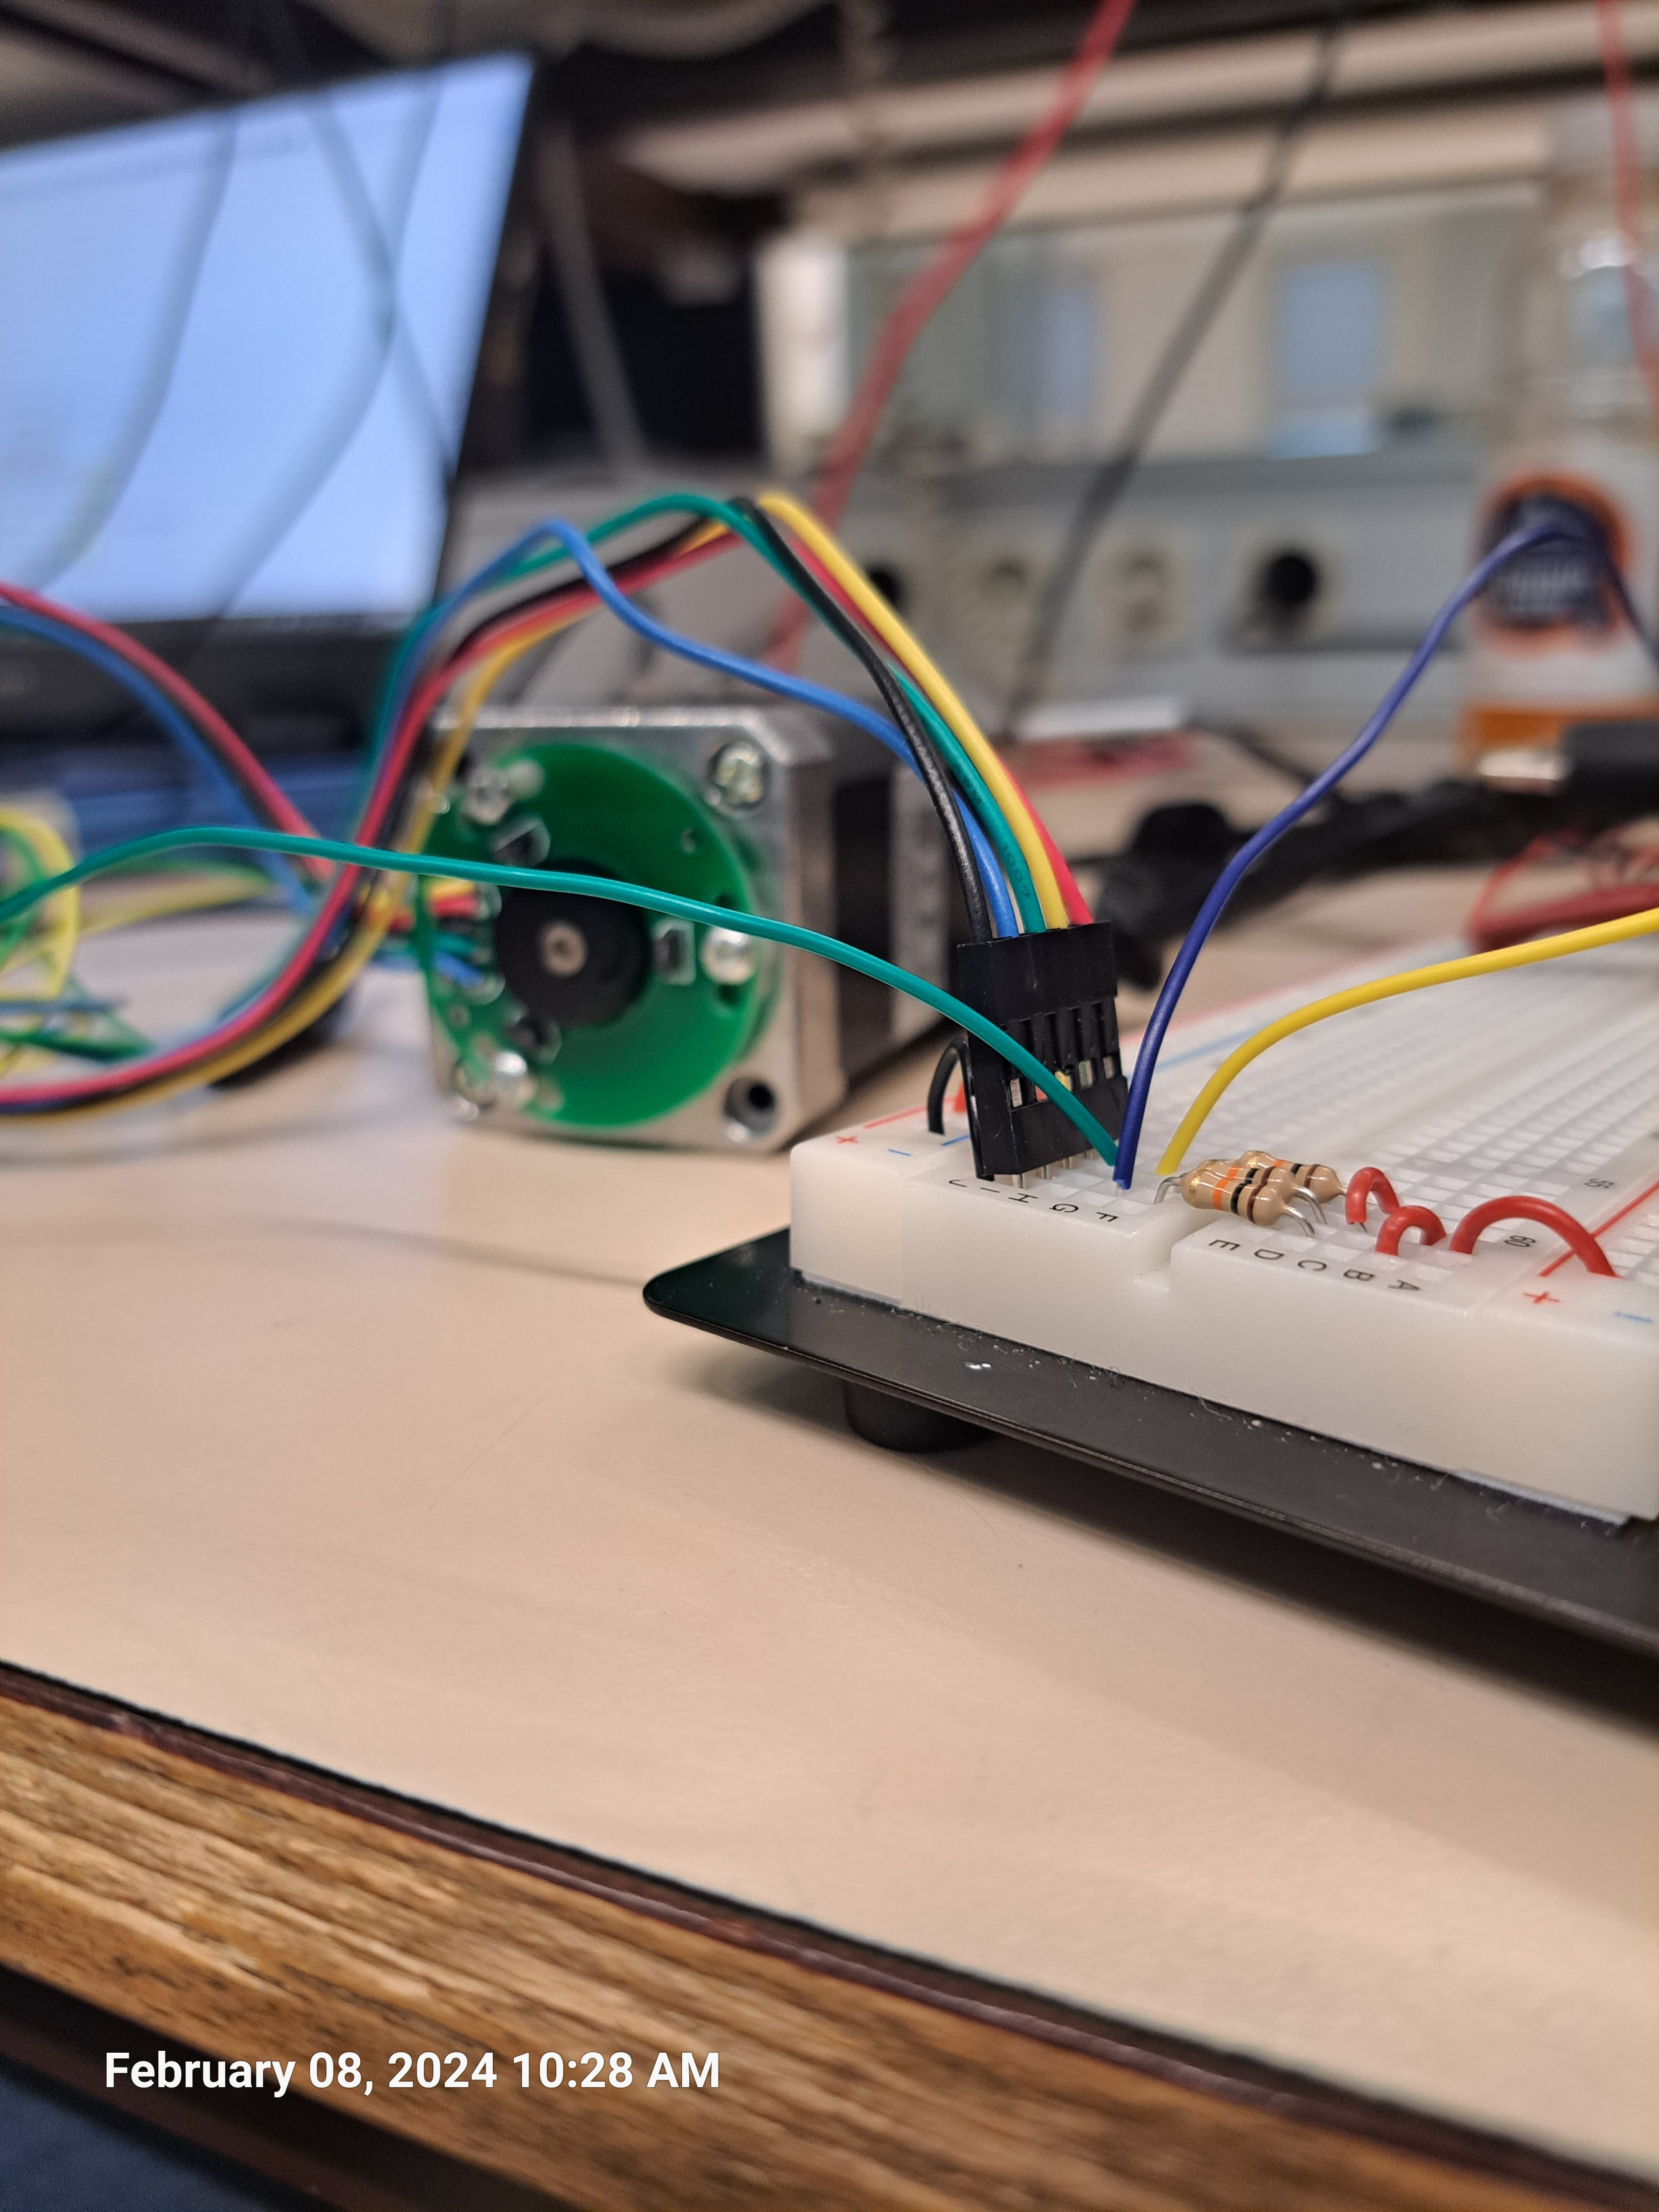
\includegraphics[width=0.3\textwidth]{img/Testing_Hallsensor_8-2-2024/Pictures/pull-up-resistor-breadboard-and-hall-sensor2.jpg}
    \caption{Wiring Diagram with Pull-up Resistors}
    \label{fig:hall_sensor_wiring_diagram}
\end{figure}

The circuit diagram, shown in \autoref{fig:hall_sensor_circuit_diagram}, illustrates the connection of the Hall sensors with the pull-up resistors.

\begin{figure}[H]
    \centering
    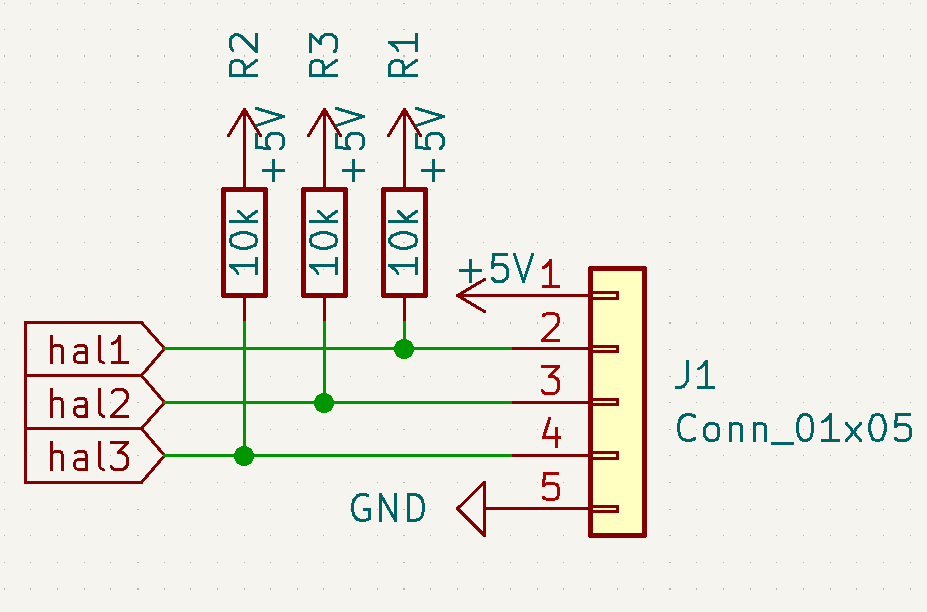
\includegraphics[width=0.45\textwidth]{img/Testing_Hallsensor_8-2-2024/Circuit/hall_sensor_circuit.png}
    \caption{Circuit: Hall sensor pinout with Pull-up Resistors}
    \label{fig:hall_sensor_circuit_diagram}
\end{figure}

Since we now understand the Hall sensor's function, its role in our application, and how to obtain stable readings, we can proceed with the software development.

\subsection{Software}
Using the Hall sensor input data we can determine the required ON/OFF states of the MOSFETS in the half bridges. This can be done using the build in HAL sensor functions as in \autoref{lst:HALFunction} or using registers as in \autoref{lst:Registers}. These listings will be further explained in \autoref{subsubsection:HALFunctions} and \autoref{subsubsection:Registers} 

The outputs from these listings are determined by \autoref{table:HallInput_Output} this is a diagram with the six Hall sensor states in time order and the output needed to the IN pin of the gate driver. The Out sections in this table contain the same data but have a different layout for better overview of the data.
\subsubsection{HAL functions}
\label{subsubsection:HALFunctions}
Using the HAL functions build into the STM32 we can with existing functions write ON/OFF states to the gate driver. This is achieved by first setting the HALPrevU - W variables on startup and after this to set the correct output equal to the previous input from the correct Hall sensor as shown in \autoref{lst:HALFunction}. For example for the output to Phase U the input from Hall W will be used. This is visualised in \autoref{table:HallInput_Output}

The benefit of using this method is simplicity and ease of use. This however comes at the cost of time, it takes significantly longer to write all necessary data than when using registers.

\subsubsection{Registers}
\label{subsubsection:Registers}
Another method to manipulate the output data to the gate driver is by directly changing the output data register of the correct GPIO port in this case port C. To load the correct data into this register the data from the input register of GPIO port B will be read an shifted to the correct pin numbers.

\autoref{lst:Registers} contains the code necessary to achieve this. First the Output Data Register (ODR) is set to the previous input data of the Hall sensors. After this the HALPrev variable will be set to the current input data shifted 8 bits to the left as the input data is on pins 5 to 7 and the output pins are 13 to 15.

The drawback of this method is the lack of simplicity. The troubleshooting and comprehending of the code will become much more difficult compared to using HAL functions.

\begin{table}[H]
\centering
\resizebox{\textwidth}{!}{%
\begin{tabular}{|ccc|c|ccc|c|ccc|}
\hline
\multicolumn{1}{|c|}{\cellcolor[HTML]{C0C0C0}\textbf{HallU}} &
  \multicolumn{1}{c|}{\cellcolor[HTML]{C0C0C0}\textbf{HallV}} &
  \cellcolor[HTML]{C0C0C0}\textbf{HallW} &
   &
  \multicolumn{1}{c|}{\cellcolor[HTML]{C0C0C0}\textbf{OutU}} &
  \multicolumn{1}{c|}{\cellcolor[HTML]{C0C0C0}\textbf{OutV}} &
  \cellcolor[HTML]{C0C0C0}\textbf{OutW} &
   &
  \multicolumn{1}{c|}{\cellcolor[HTML]{C0C0C0}\textbf{OutW}} &
  \multicolumn{1}{l|}{\cellcolor[HTML]{C0C0C0}\textbf{OutU}} &
  \multicolumn{1}{l|}{\cellcolor[HTML]{C0C0C0}\textbf{OutV}} \\ \cline{1-3} \cline{5-7} \cline{9-11} 
\multicolumn{1}{|c|}{1} &
  \multicolumn{1}{c|}{0} &
  1 &
   &
  \multicolumn{1}{c|}{0} &
  \multicolumn{1}{c|}{1} &
  0 &
   &
  \multicolumn{1}{c|}{0} &
  \multicolumn{1}{c|}{0} &
  1 \\ \cline{1-3} \cline{5-7} \cline{9-11} 
\multicolumn{1}{|c|}{1} &
  \multicolumn{1}{c|}{0} &
  0 &
   &
  \multicolumn{1}{c|}{0} &
  \multicolumn{1}{c|}{1} &
  1 &
   &
  \multicolumn{1}{c|}{1} &
  \multicolumn{1}{c|}{0} &
  1 \\ \cline{1-3} \cline{5-7} \cline{9-11} 
\multicolumn{1}{|c|}{1} &
  \multicolumn{1}{c|}{1} &
  0 &
   &
  \multicolumn{1}{c|}{0} &
  \multicolumn{1}{c|}{0} &
  1 &
   &
  \multicolumn{1}{c|}{1} &
  \multicolumn{1}{c|}{0} &
  0 \\ \cline{1-3} \cline{5-7} \cline{9-11} 
\multicolumn{1}{|c|}{0} &
  \multicolumn{1}{c|}{1} &
  0 &
   &
  \multicolumn{1}{c|}{1} &
  \multicolumn{1}{c|}{0} &
  1 &
   &
  \multicolumn{1}{c|}{1} &
  \multicolumn{1}{c|}{1} &
  0 \\ \cline{1-3} \cline{5-7} \cline{9-11} 
\multicolumn{1}{|c|}{0} &
  \multicolumn{1}{c|}{1} &
  1 &
   &
  \multicolumn{1}{c|}{1} &
  \multicolumn{1}{c|}{0} &
  0 &
   &
  \multicolumn{1}{c|}{0} &
  \multicolumn{1}{c|}{1} &
  0 \\ \cline{1-3} \cline{5-7} \cline{9-11} 
\multicolumn{1}{|c|}{0} &
  \multicolumn{1}{c|}{0} &
  1 &
   &
  \multicolumn{1}{c|}{1} &
  \multicolumn{1}{c|}{1} &
  0 &
   &
  \multicolumn{1}{c|}{0} &
  \multicolumn{1}{c|}{1} &
  1 \\ \cline{1-3} \cline{5-7} \cline{9-11} 
\multicolumn{3}{|c|}{\cellcolor[HTML]{EFEFEF}\textit{Hall}} &
  \multirow{-8}{*}{} &
  \multicolumn{3}{c|}{\cellcolor[HTML]{EFEFEF}\textit{Out}} &
  \multirow{-8}{*}{} &
  \multicolumn{3}{c|}{\cellcolor[HTML]{EFEFEF}\textit{Out}} \\ \hline
\end{tabular}%
}
\caption{Hall Input Output Diagram}
\label{table:HallInput_Output}
\end{table}

\begin{lstlisting}[caption={Set MOSFET ON/OFF states using HAL functions},label={lst:HALFunction},language=C]
    // Set new MOSFETS states
	HAL_GPIO_WritePin(GPIOC, GPIO_PIN_13, HALPrevW); // Set output U to previous HAL state W
	HAL_GPIO_WritePin(GPIOC, GPIO_PIN_14, HALPrevU); // Set output V to previous HAL state U
	HAL_GPIO_WritePin(GPIOC, GPIO_PIN_15, HALPrevV); // Set output W to previous HAL state V
	
	HALPrevU = HAL_GPIO_ReadPin(GPIOB, GPIO_PIN_5);
	HALPrevV = HAL_GPIO_ReadPin(GPIOB, GPIO_PIN_6);
	HALPrevW = HAL_GPIO_ReadPin(GPIOB, GPIO_PIN_7);	
\end{lstlisting}

\begin{lstlisting}[caption={Set MOSFET ON/OFF states using registers},label={lst:Registers},language=C]
    // Set new MOSFET states
    GPIOC->ODR |= HALPrev;
	HALPrev = GPIOB->IDR << 8;
\end{lstlisting}

